\documentclass{article}

\usepackage[T1]{fontenc}    %Schriftart des Dokumentes
\usepackage[ngerman]{babel} %Dokumentensprache, hier Deutsch
\usepackage{amsmath, amssymb, stmaryrd} %mathematische Schriftzeichen
\usepackage{graphicx} %Einfügen von Grafiken
\usepackage{wrapfig}
\usepackage{bm}
\usepackage{subfig}
\usepackage{newclude}
\usepackage{pdfpages}

\setlength{\parindent}{0pt} %Einrückung von Absätzen auf null gesetzt
\setlength{\parskip}{10pt} %Abstand zischen Absätzen auf 10pt gesetzt

\title{Versuch 256: Röntgenfluoreszenz}
\author{Matthias Kuntz}
\date{29.04.2024}

\renewcommand*\contentsname{Zusammenfassung}

\begin{document}

\maketitle

\tableofcontents

\newpage

%-------------------------EINLEITUNG-------------------------
\section{Einleitung}

Eine häufig verwendete Eigenschaft von Röntgenstrahlung ist die Emission charakteristischer Linien bei der Bestrahlung eines Materials. Diese Linien, die für jedes Element anders und somit eindeutig sind, können analysiert und untersucht werden um so Informationen über die Zusammensetzung eines Objekts zu erlangen. Alternativ kann man die Linien bei bekannten Proben vermessen, um physikalische Konstanten wie die Rydbergenergie zu bestimmen. In diesem Versuch soll es um die Röntgenfluoreszenz gehen, welche sich genau all das zunutze macht, um mit verschiedenen Proben über das Moseley'sche Gesetz die Rydbergenergie zu bestimmen und die Zusammensetzung unbekannter Testobjekte zu untersuchen.  

\subsection{Physikalische Grundlagen}

\subsubsection{Röntgenfuoreszenz}

Beim Aufprall von Röntgenstrahlung auf Materie entsteht durch den Abfall von Elektronen aus höheren Schalen zu den von der Strahlung freigemachten Stellen eine charakteristische materialabhängige Strahlung, welche als Röntgenfluoreszenz bezeichnet wird. Die Energie der Strahlung $\Delta E$ beim Übergang von der Schale mit Hauptquantenzahl $n_2$ auf $n_1$ wird über das Bohr'sche Atommodell folgendermaßen approximiert:

\begin{equation}
    \Delta E = E_2 - E_1 = ch R_\infty \left( \frac{(Z - \sigma_{n_1})^2}{n_1^2} - \frac{(Z - \sigma_{n_2})^2}{n_2^2} \right).
\end{equation}

Hierbei stehen $c$ und $h$ für Lichtgeschwindigkeit sowie Planck'sches Wirkungsquantum, $Z$ für die Kernladungszahl und $R_\infty$ die Rydbergkonstante. Die Abschirmkonstanten $\sigma_i$ berücksichtigen die Abschwächung der effektiven Kernladungszahl, welche von den Elektronen verspürt wird, im Vergleich zur gesamten und können näherungsweise zu einer Konstanten $\sigma_{12}$ zusammengefasst werden:

\begin{equation}
    \Delta E = ch R_\infty (Z - \sigma_{12})^2 \left( \frac{1}{n_1^2} - \frac{1}{n_2^2} \right).
\end{equation}

Mit der Rydbergenergie $E_R = ch R_\infty \approx 13,6$eV erhält man das Moseley'sche Gesetz

\begin{equation}
    \sqrt{\frac{E}{E_R}} =(Z - \sigma_{12}) \sqrt{ \frac{1}{n_1^2} - \frac{1}{n_2^2}},
\end{equation}

welches sich bei der K$_\alpha$-Strahlung bei nicht allzu schweren Kernen mit der Näherung $\sigma_{12} \approx 1$ vereinfacht zu:

\begin{equation}
    \sqrt{\frac{E}{E_R}} =(Z - 1) \sqrt{ \frac{3}{4}}.
\end{equation}


\subsubsection{Röntgenenergiedetektor}

Ein Röntgenenergiedetektor nutzt den pn-Übergang, zu sehen in Abbildung \ref{fig:pn-übergang}, welcher beim Zusammenbringen eines n-Halbleiters mit einem Überschuss an freien Elektronen und einem p-Halbleiter mit Überschuss an freien Elektronfehlstellen entsteht. Beim Zusammenbringen der beiden Halbleiter entsteht aufgrund von Diffusion und Rekombination eine neutral geladene Verarmungszone beschränkt durch das entgegenwirkende elektrische Feld der Ladungsverschiebung. Schließt man nun eine Spannung an, so vergrößert sich die Verarmungszone und Ladung, die entsteht wenn ein Röntgenphoton auf die Verarmungszone trifft und ein Photoelektron aussendet, wird durch das anliegende Feld abgesaugt, woraufhin sie von einem ladungsempfindlichen Verstärker gemessen werden kann. Die generierten Signale sind dabei proportional zur Energie der Röntgenphotonen und können von einem Vielkanalanalysator in ihrer Stärke und Häufigkeit aufgezeichnet werden, sodass ein Histogramm erstellt werden kann. Zur effektiven Analyse wird eine Energiekalibrierung durchgefüht, indem das Energiespektrum eines bekannten Elements aufgezeichnet wird. 

\phantom{.}

\begin{figure}[!h]
    \centering
    \resizebox{0.9\textwidth}{!}{
    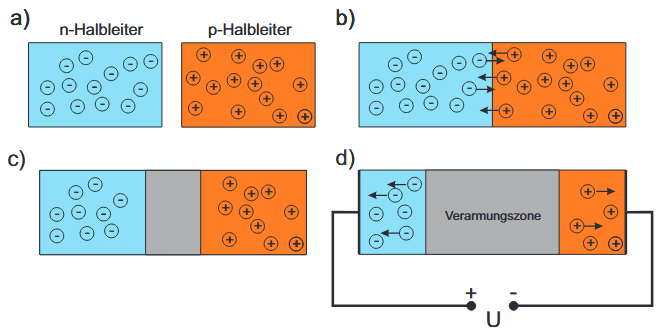
\includegraphics{graphics/pn-übergang.png}}
    \caption{pn-Übergang [Quelle: PAP2.1 Skript, S.97, Stand: 09.05.2024]}
    \label{fig:pn-übergang}
\end{figure}

\clearpage
\newpage

\subsection{Versuchsaufbau}

Der Aufbau besteht aus einem Röntgengerät mit Röntgenröhre und ist zum Großteil in Abbildung \ref{fig:aufbau} zu sehen. Die von der Röntgenröhre generierte Röntgenstrahlung wird über einen im 45°-Winkel gedrehten Tisch, auf dem verschiedene Proben platziert werden können, zu dem darüber hängenden Röntgenenergiedetektor geleitet. Dieser sendet das Signal über den Verstärker an den Vielkanalanalysator, welcher an einen Computer angeschlossen ist. Auf dem Computer dient das Programm CASSY Lab 2 zum auswerten der Daten und dem Erstellen der Histogramme. 

\phantom{.}

\begin{figure}[!h]
    \centering
    \resizebox{0.9\textwidth}{!}{
    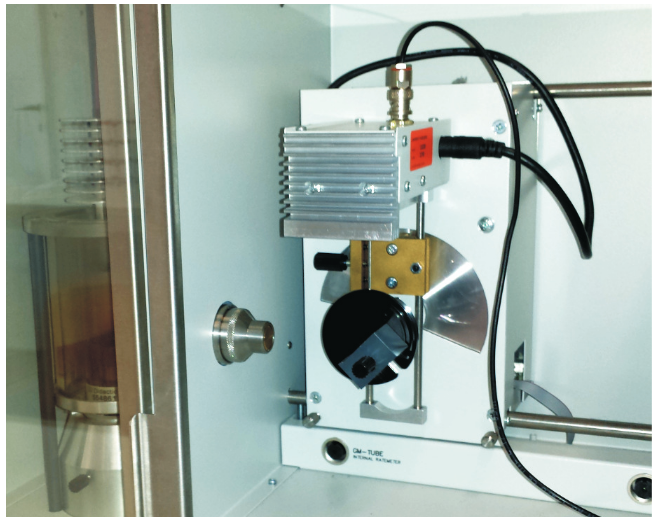
\includegraphics{graphics/aufbau256.png}}
    \caption{Versuchsaufbau [Quelle: PAP2.1 Skript, S.95, Stand: 09.05.2024]}
    \label{fig:aufbau}
\end{figure}


%---------------VERSUCHSPROTOKOLL MIT MESSDATEN---------------
\newpage

\section{Versuchsprotokoll mit Messdaten}

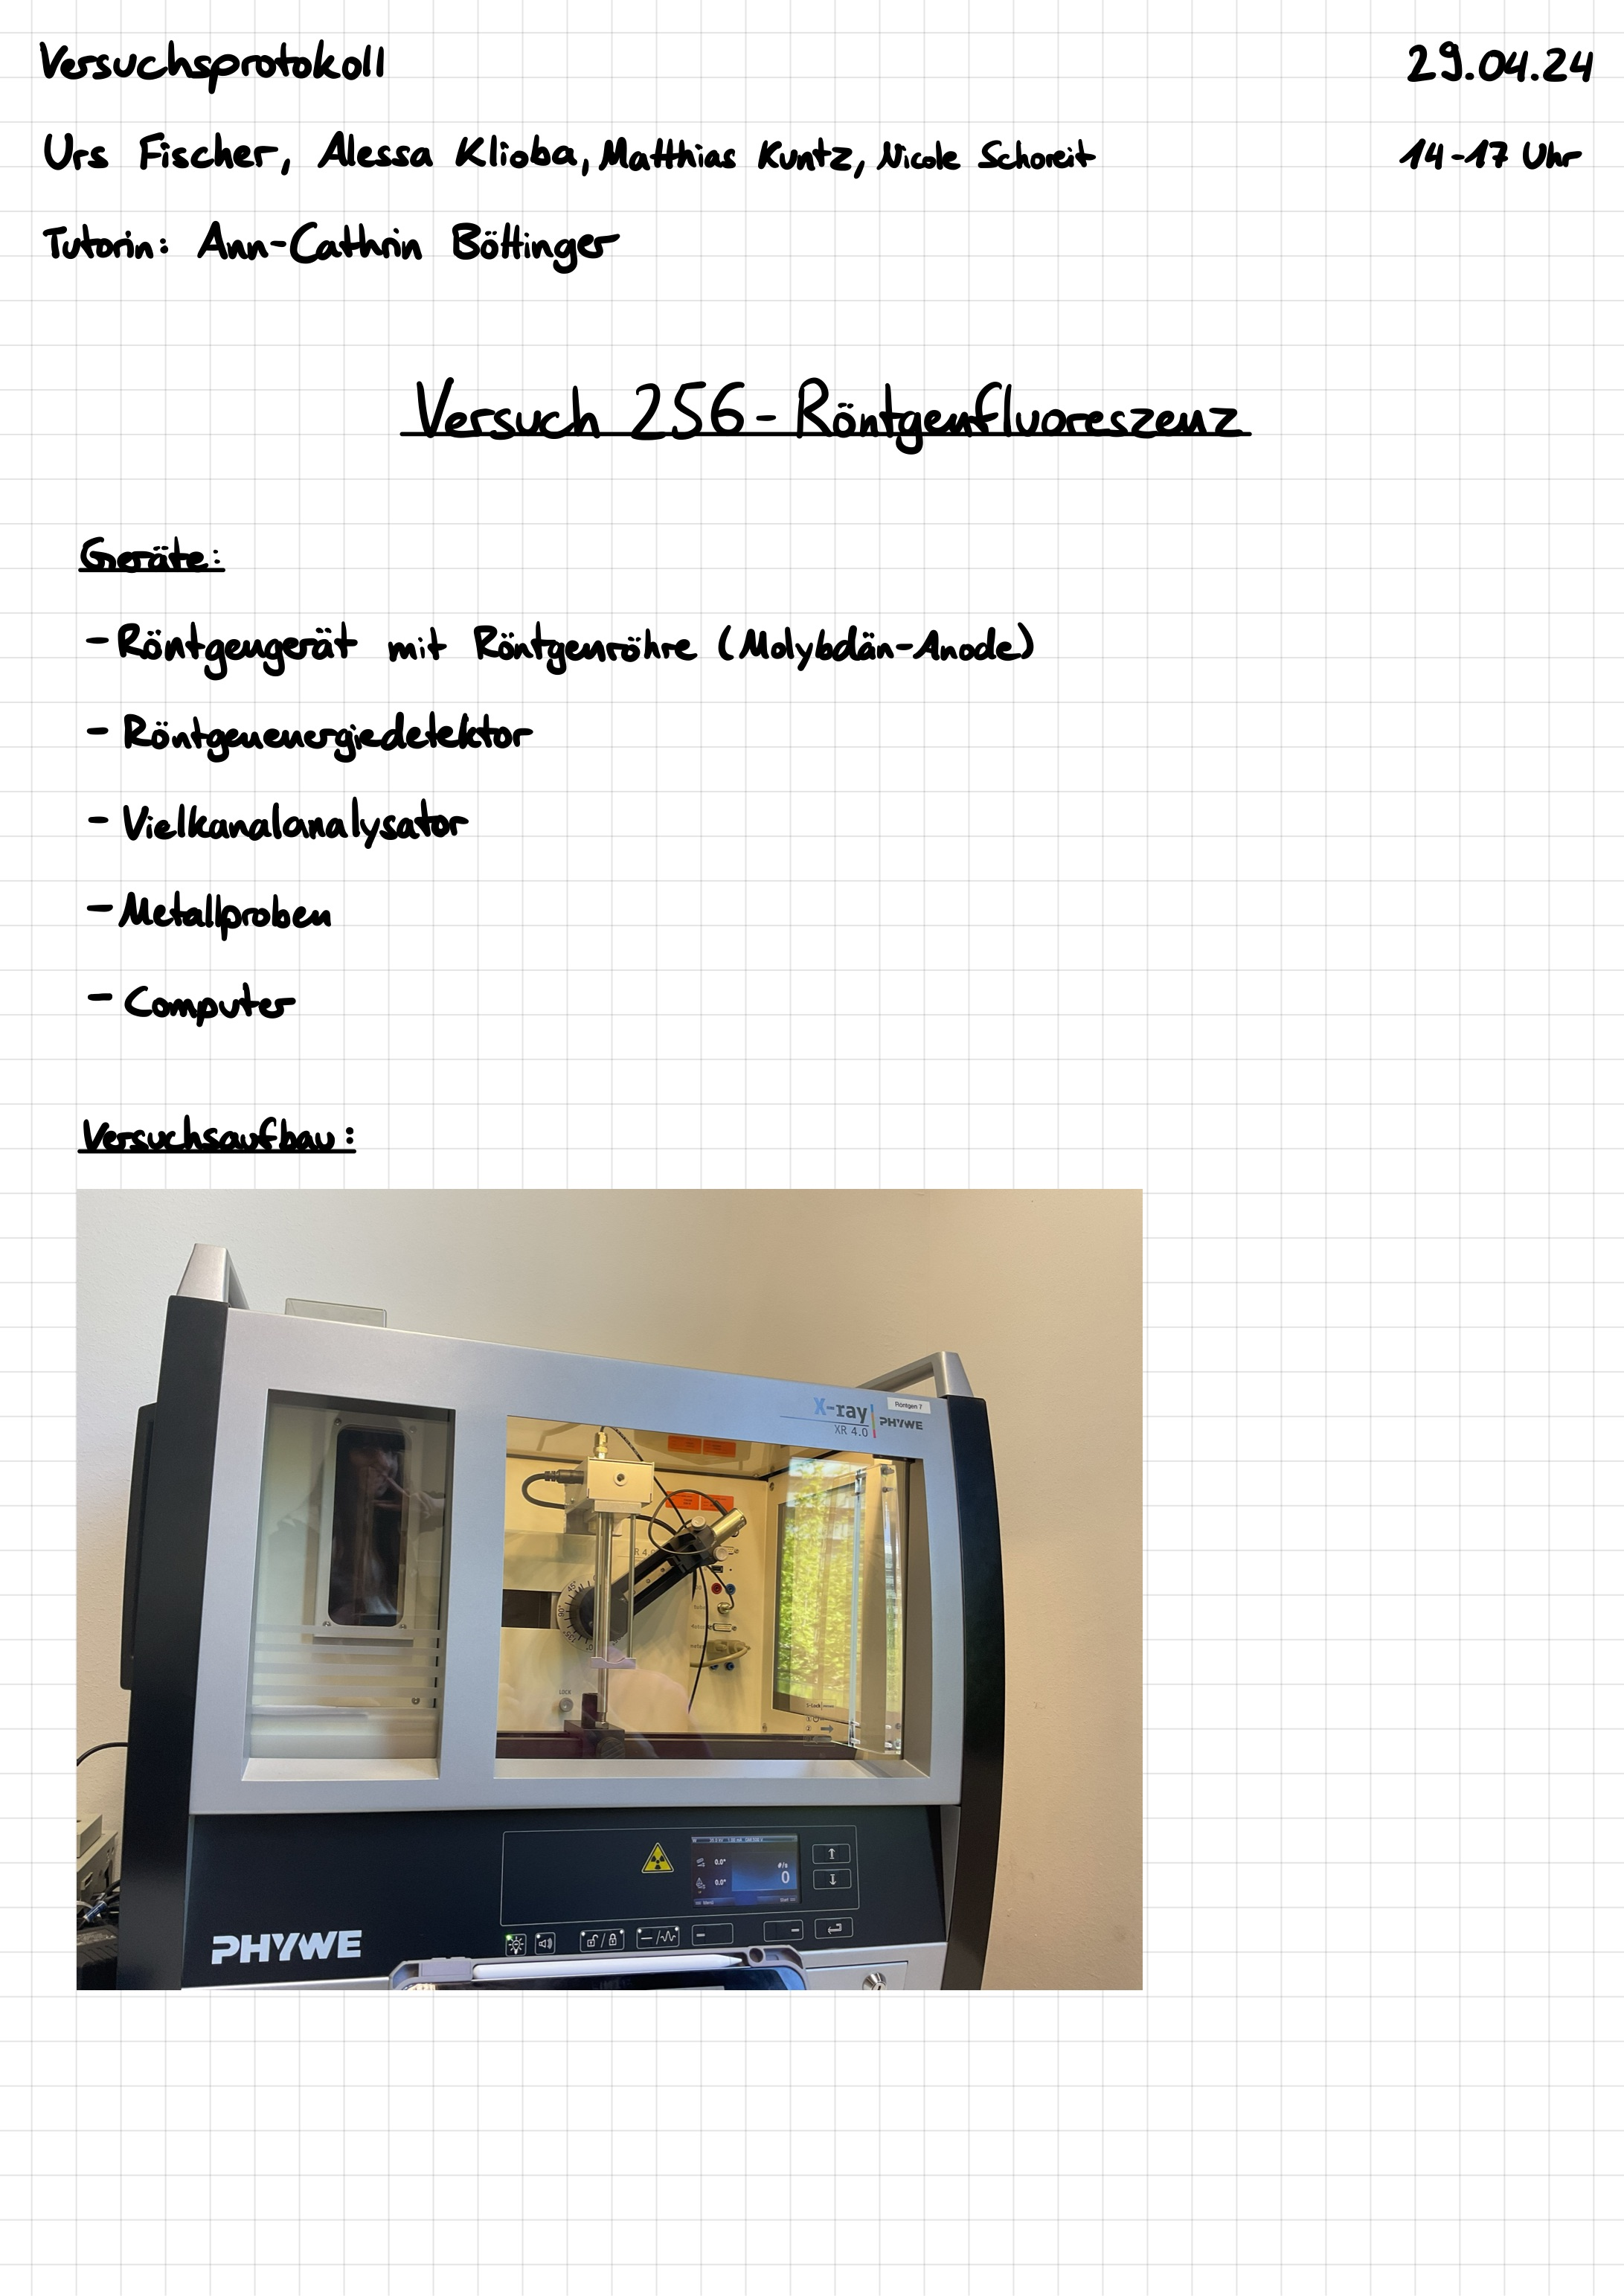
\includegraphics[width=\textwidth]{graphics/mess1.jpg}
\newpage
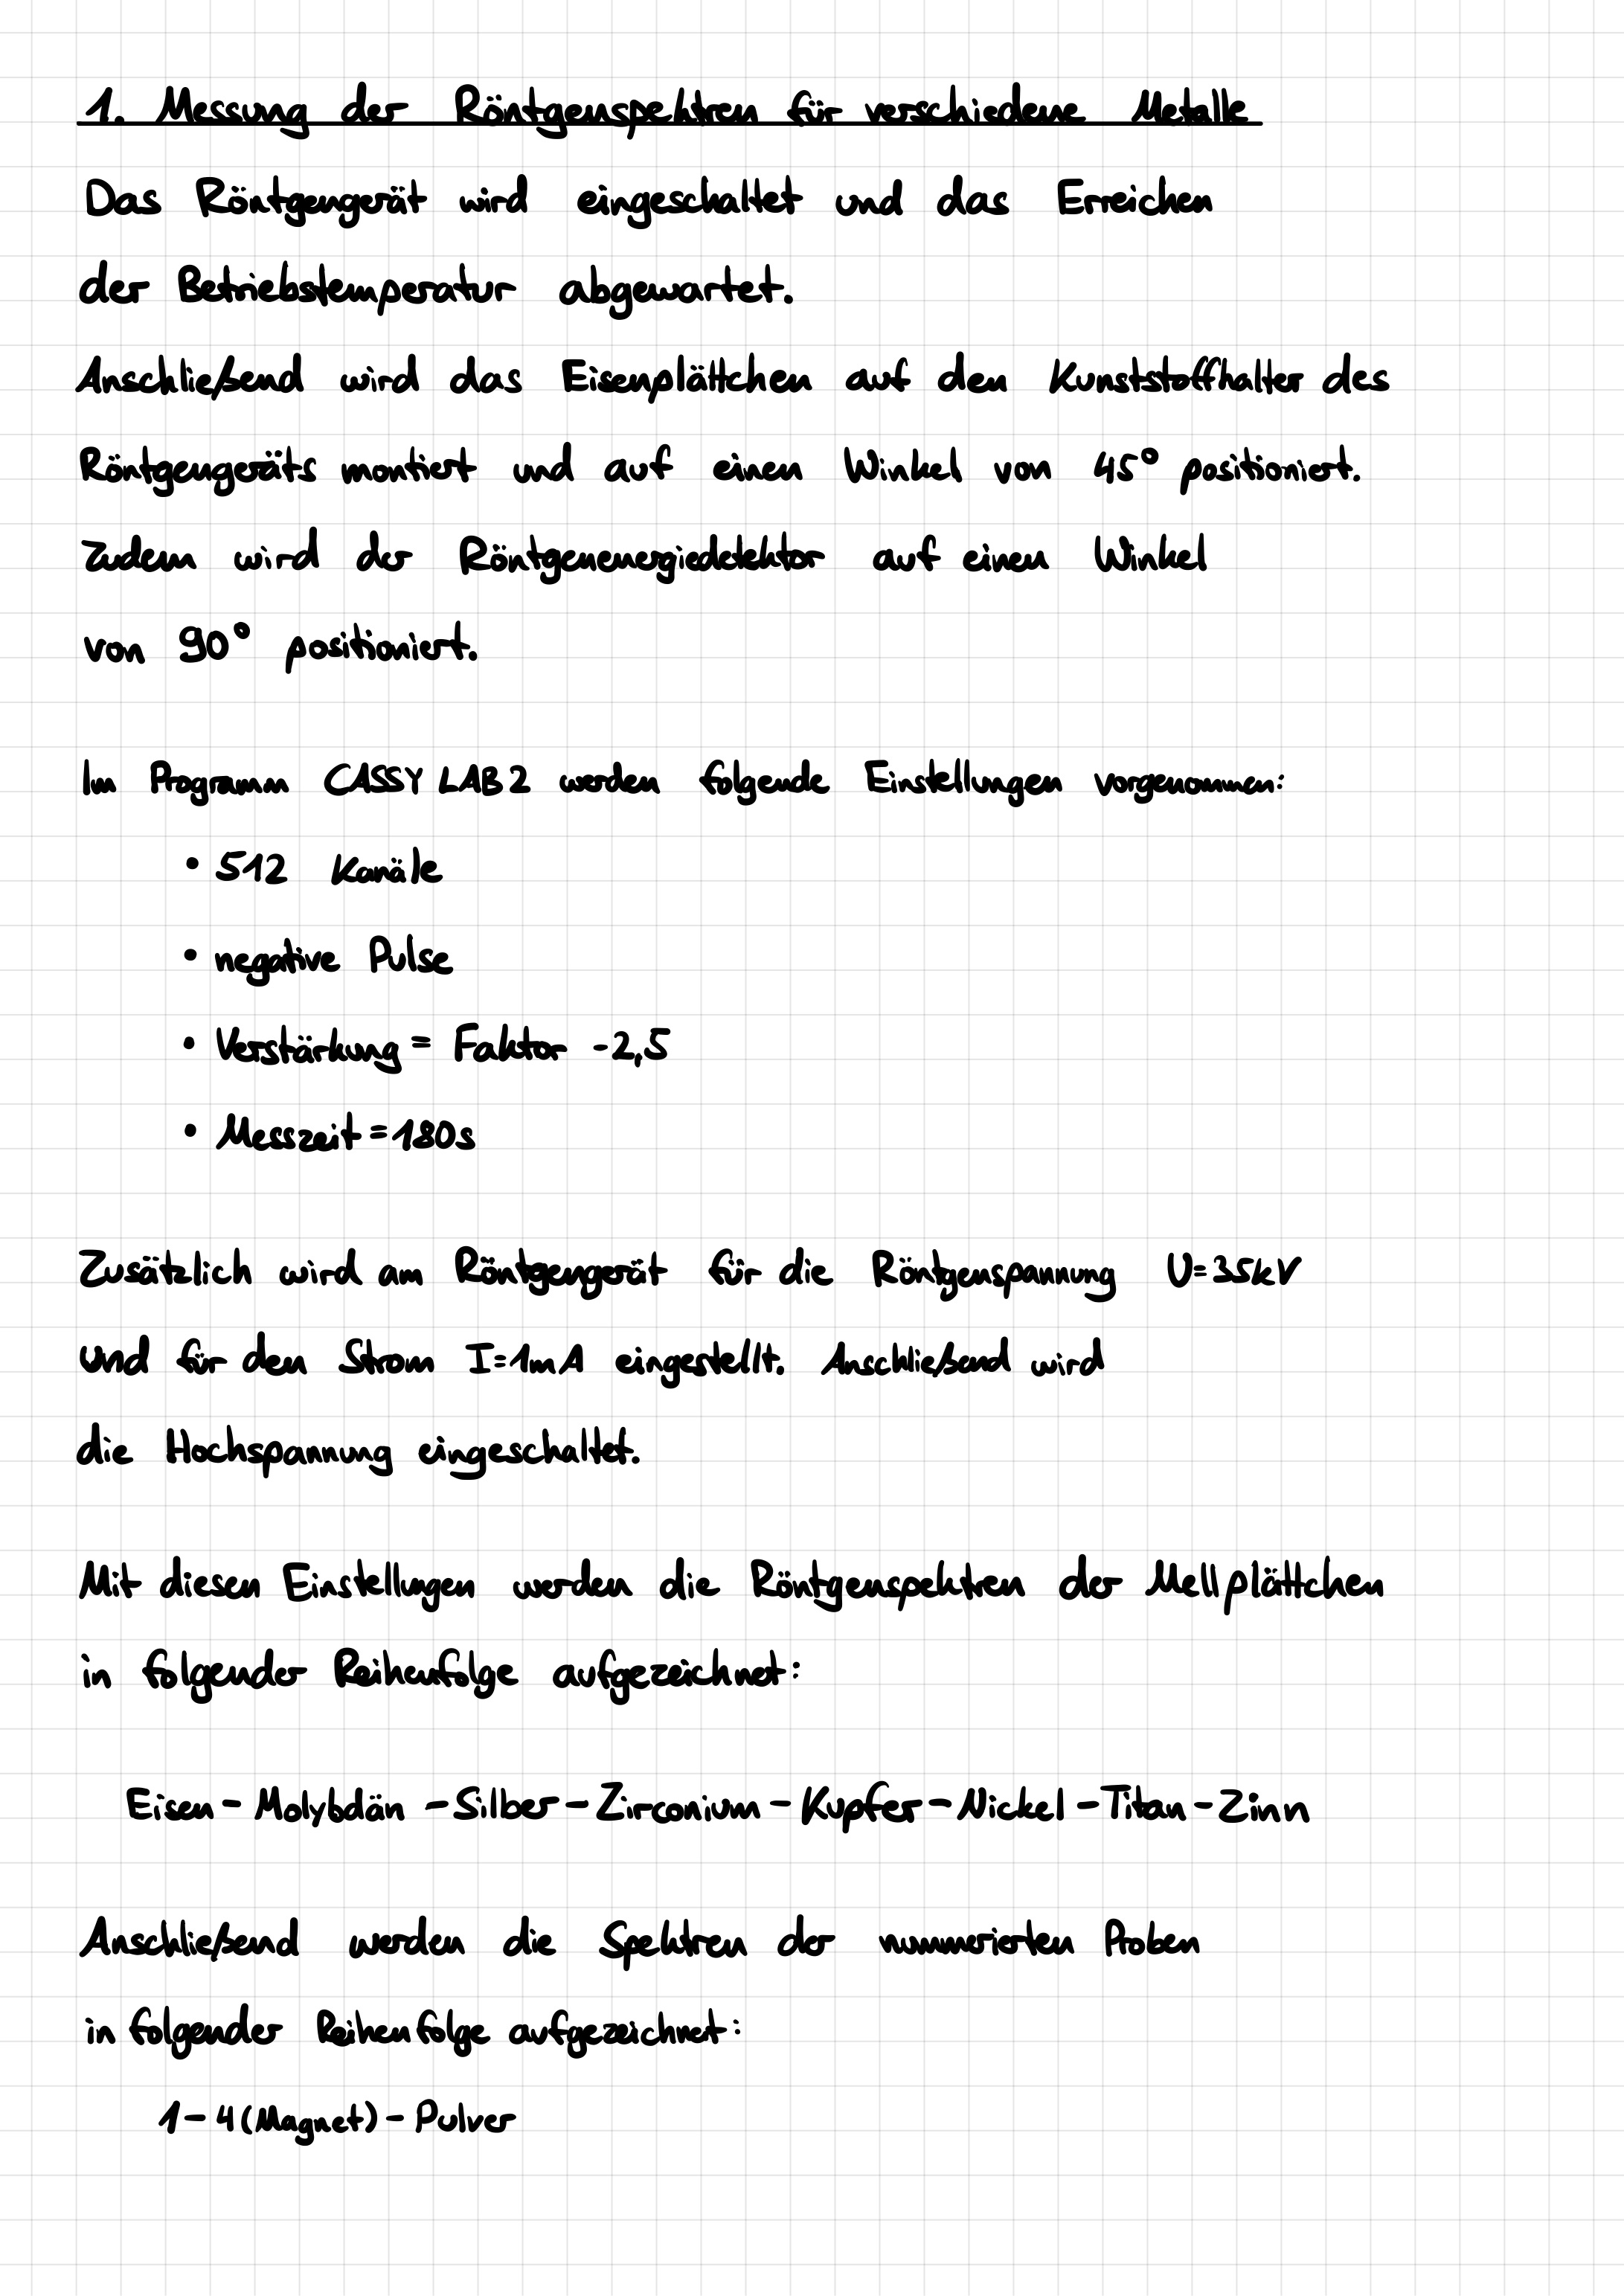
\includegraphics[width=\textwidth]{graphics/mess2.jpg}
\newpage
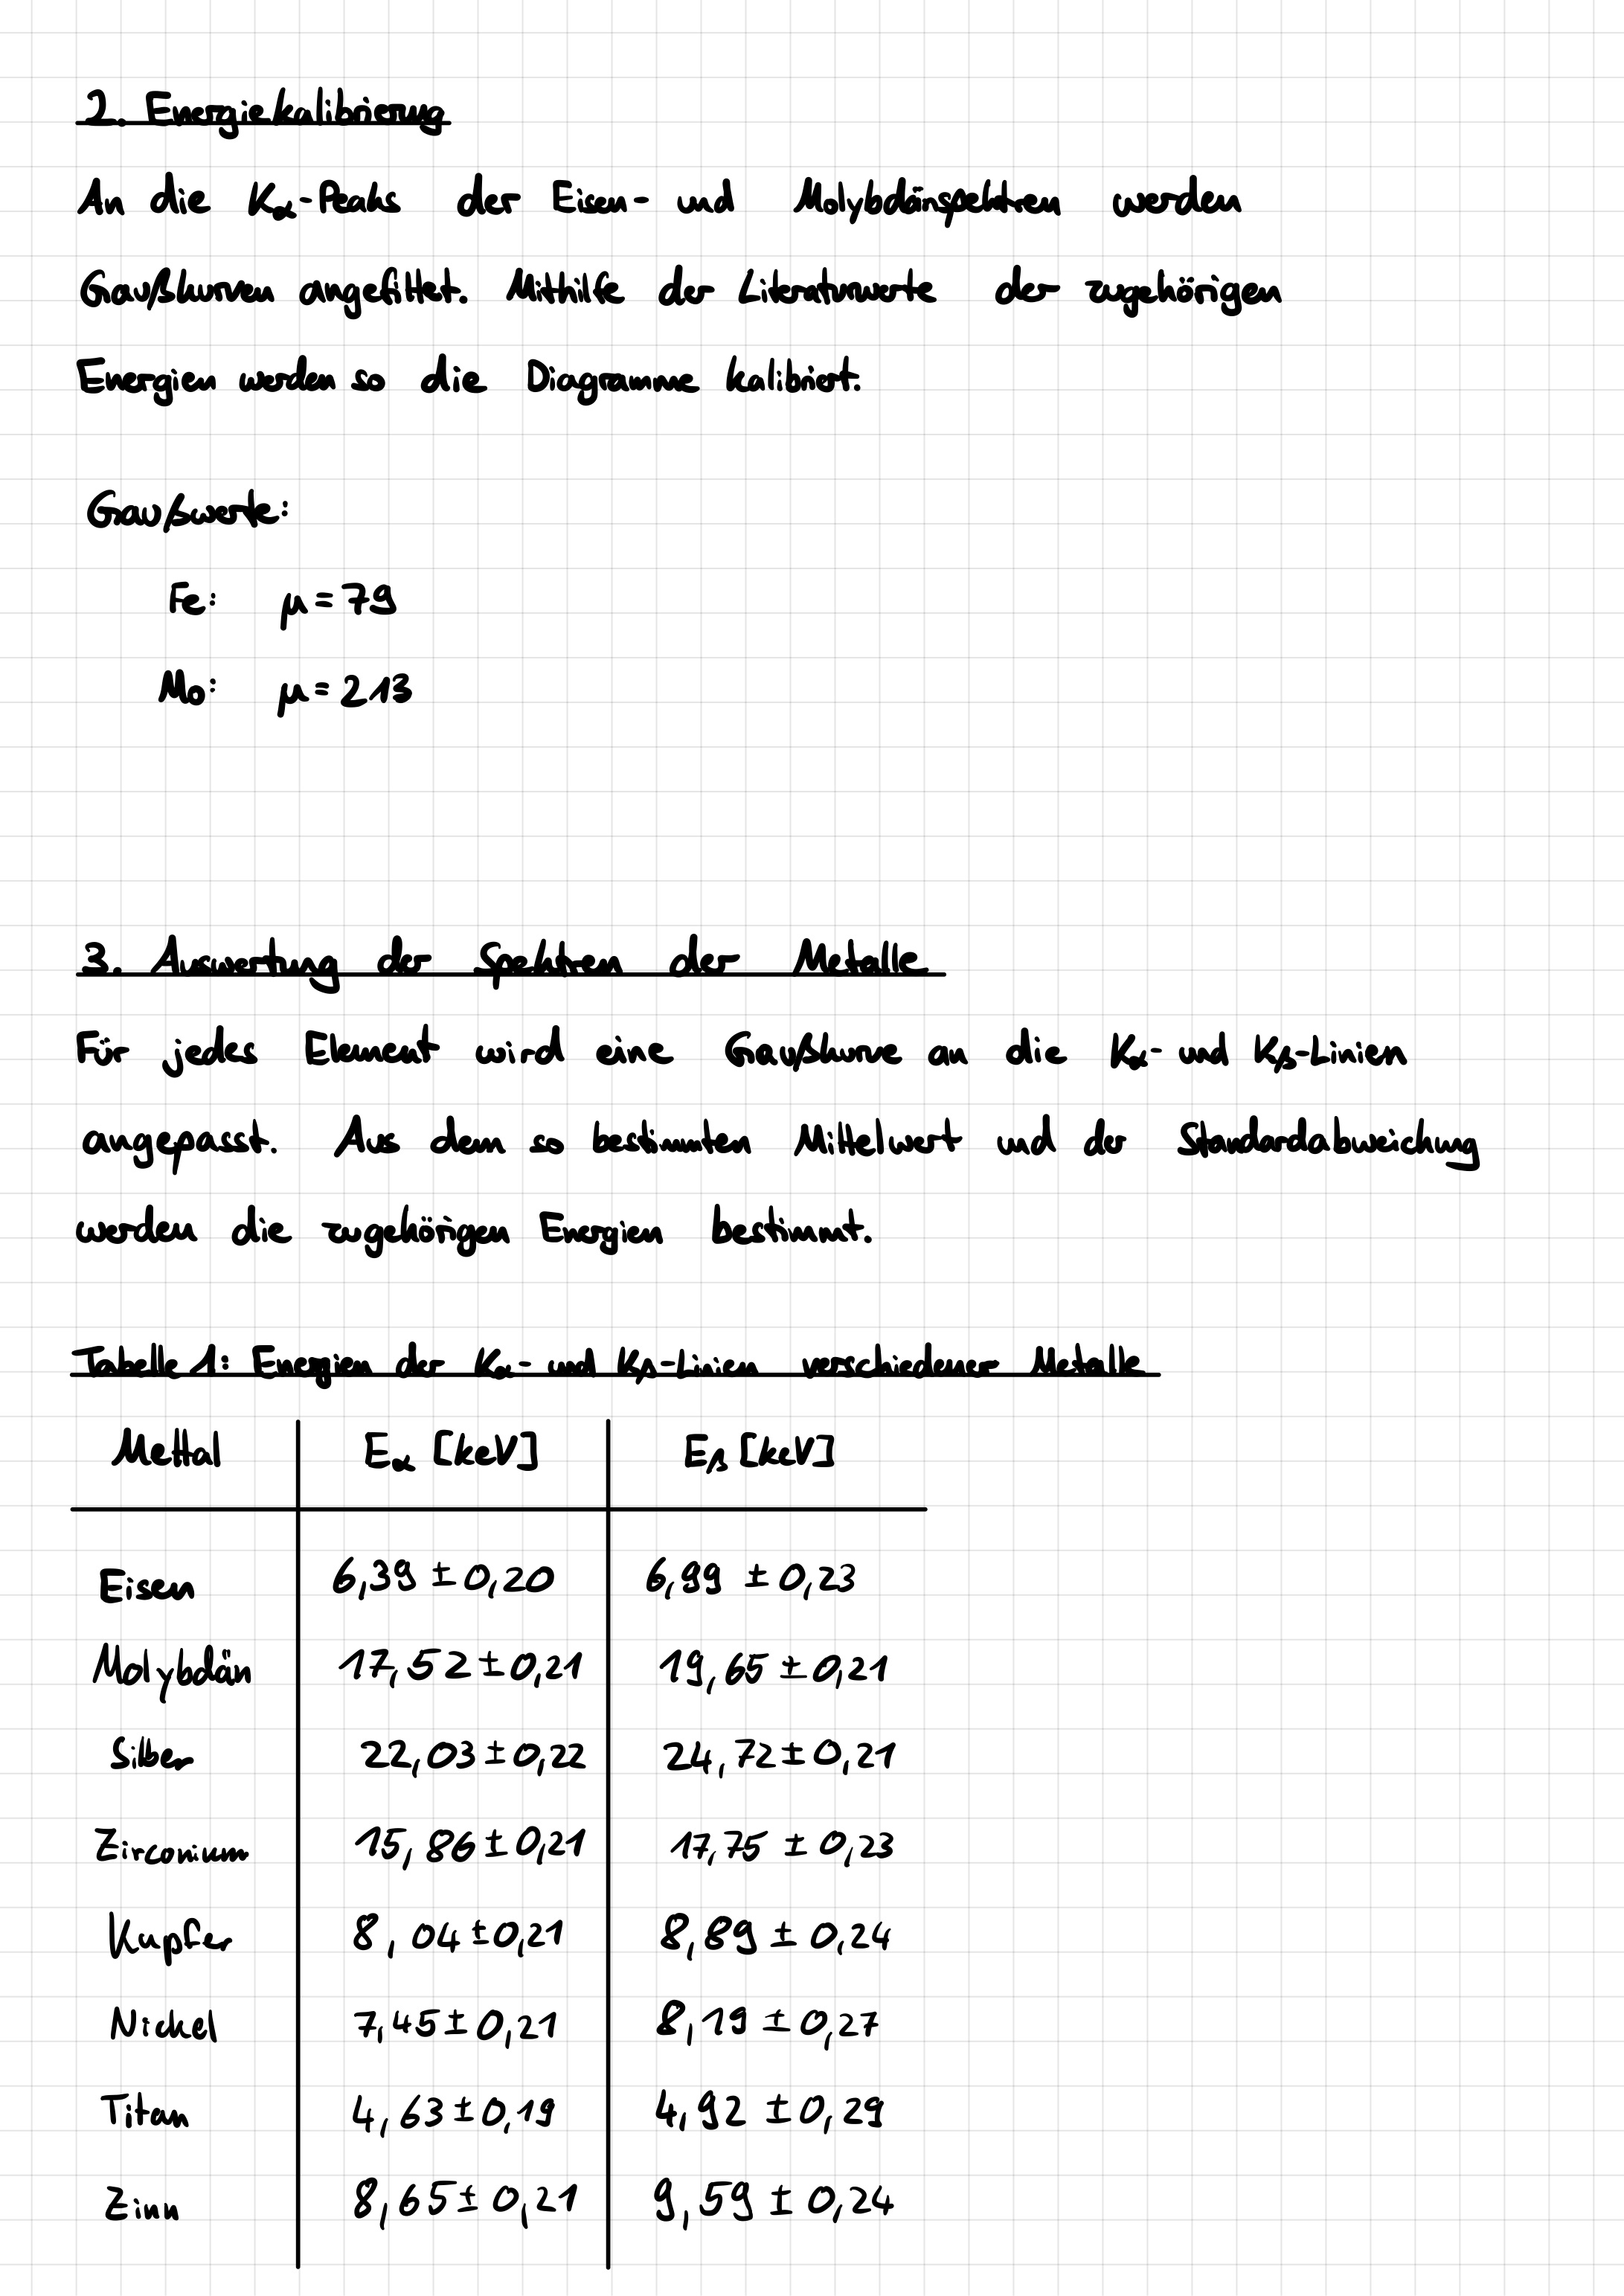
\includegraphics[width=\textwidth]{graphics/mess3.jpg}
\newpage
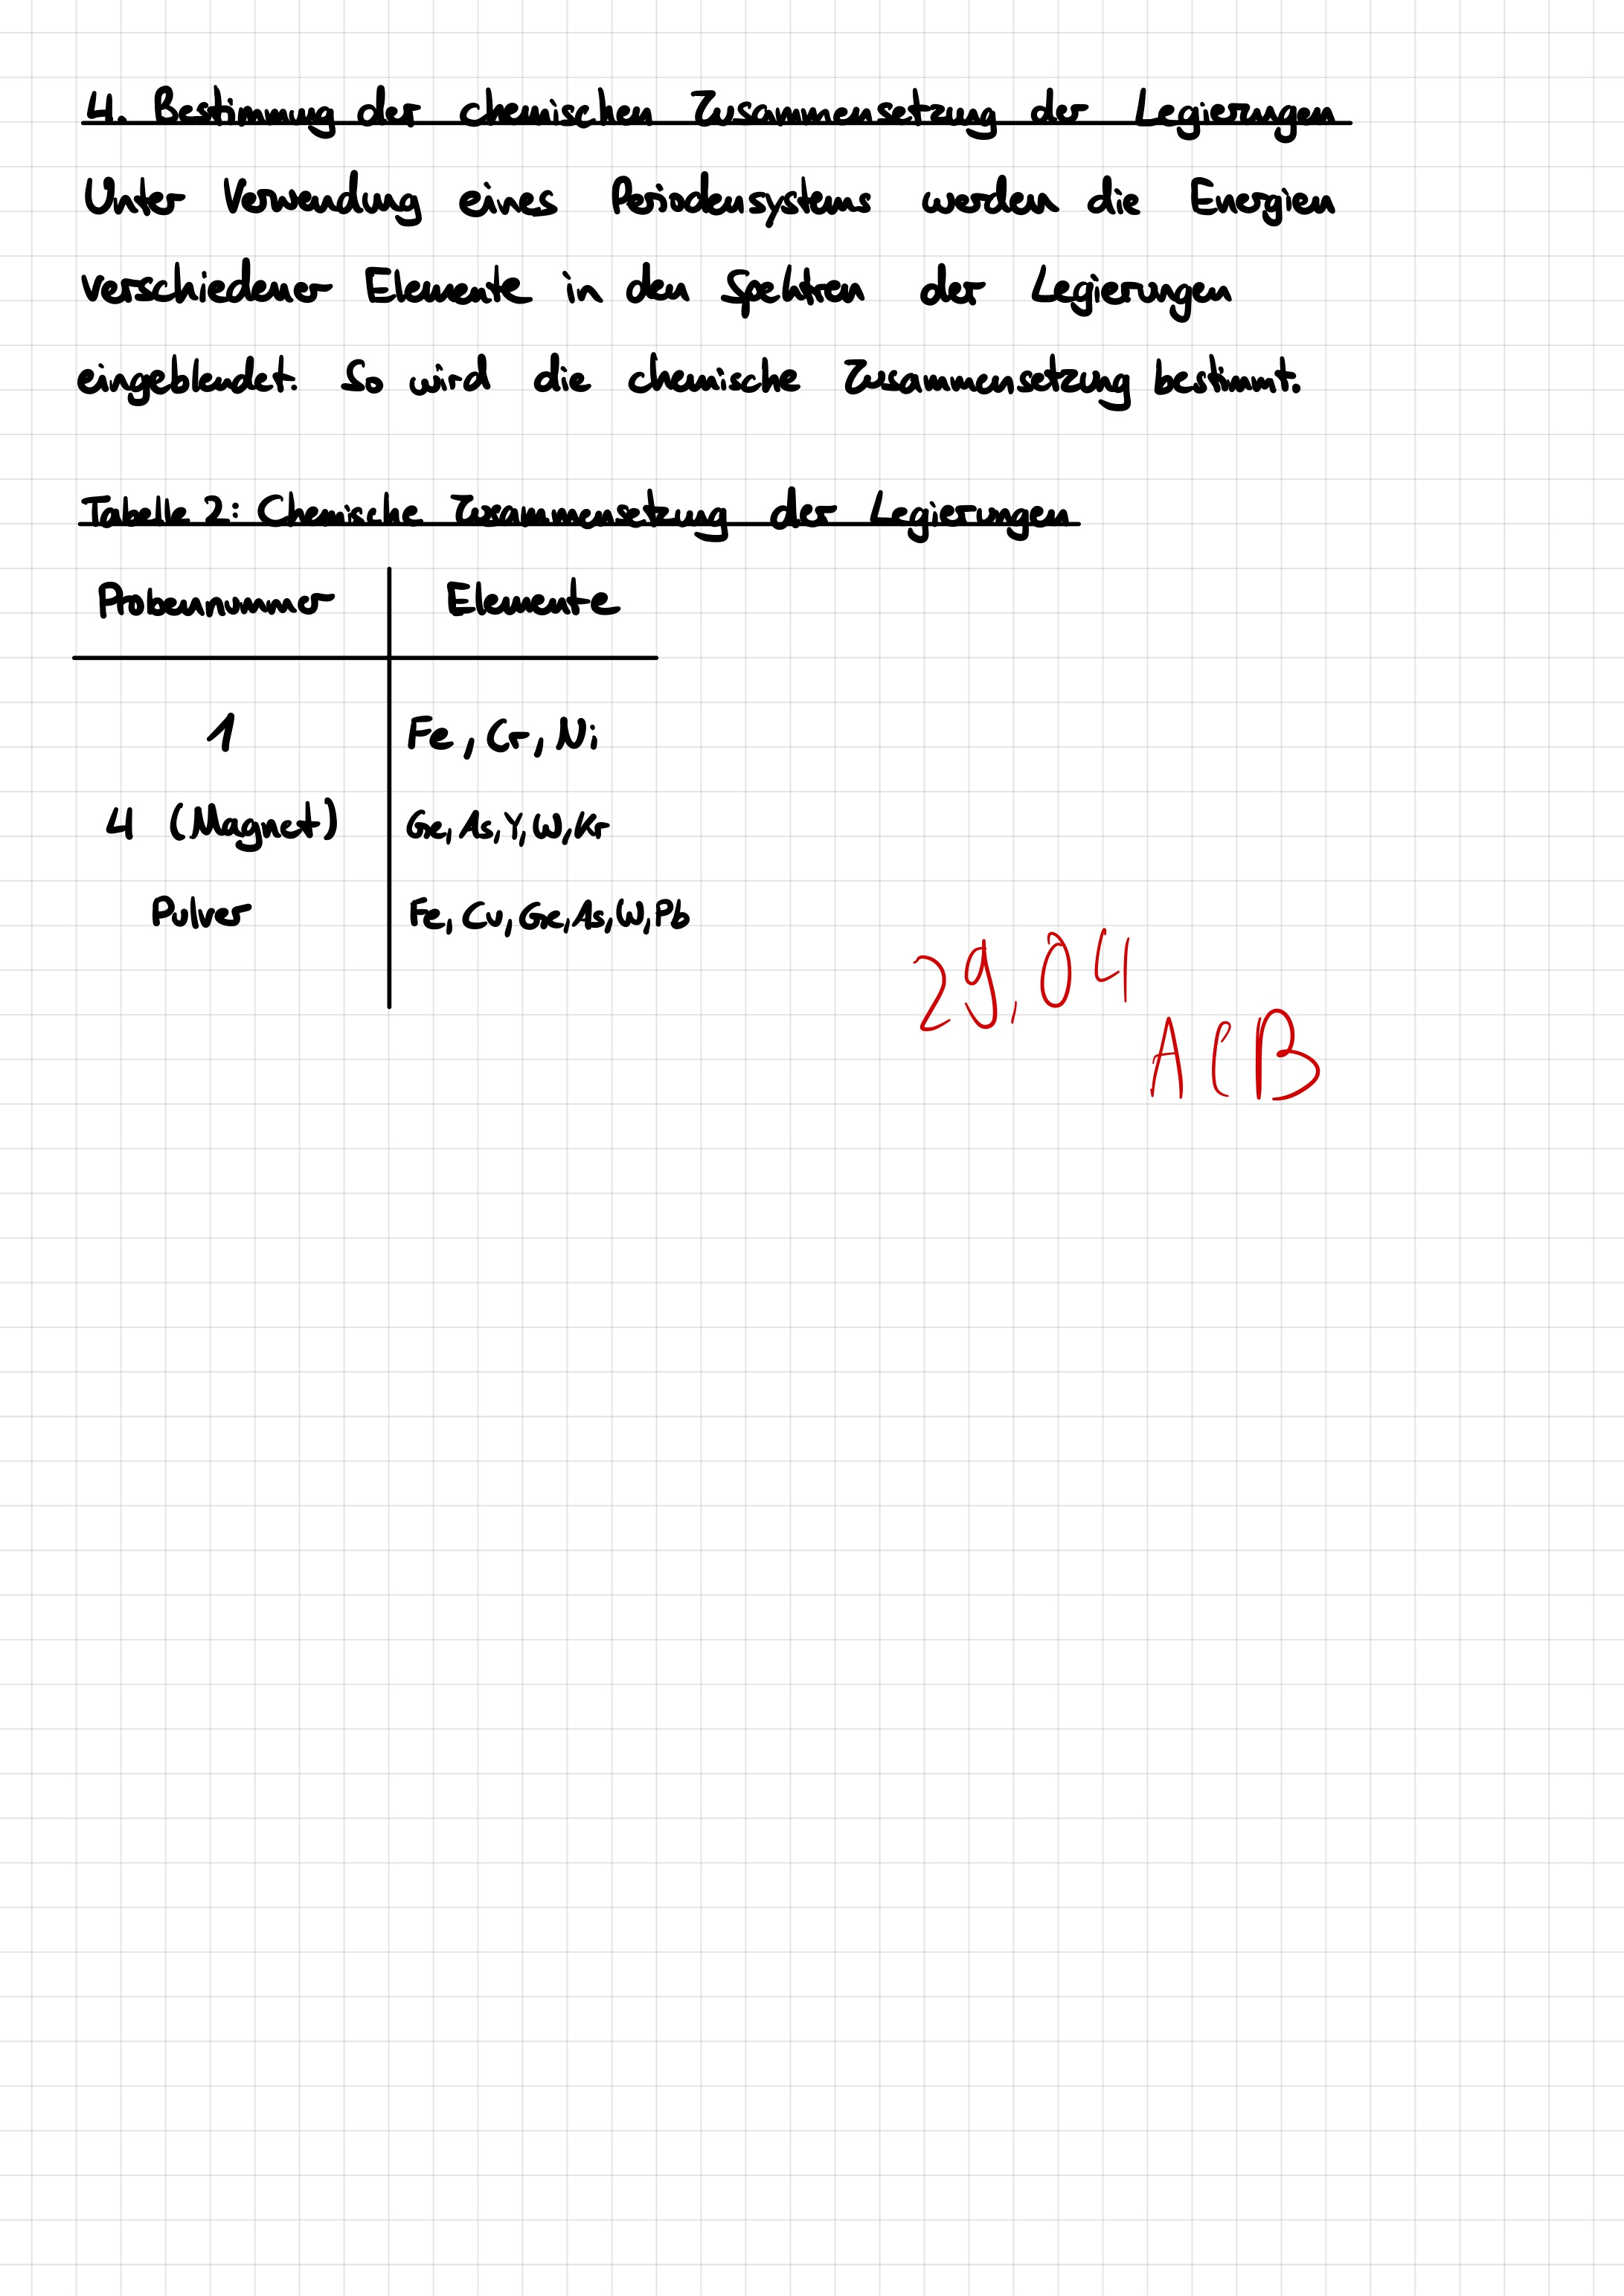
\includegraphics[width=\textwidth]{graphics/mess4.jpg}
\newpage

\begin{figure}[!p]
    \centering
    \resizebox{\textwidth}{!}{
    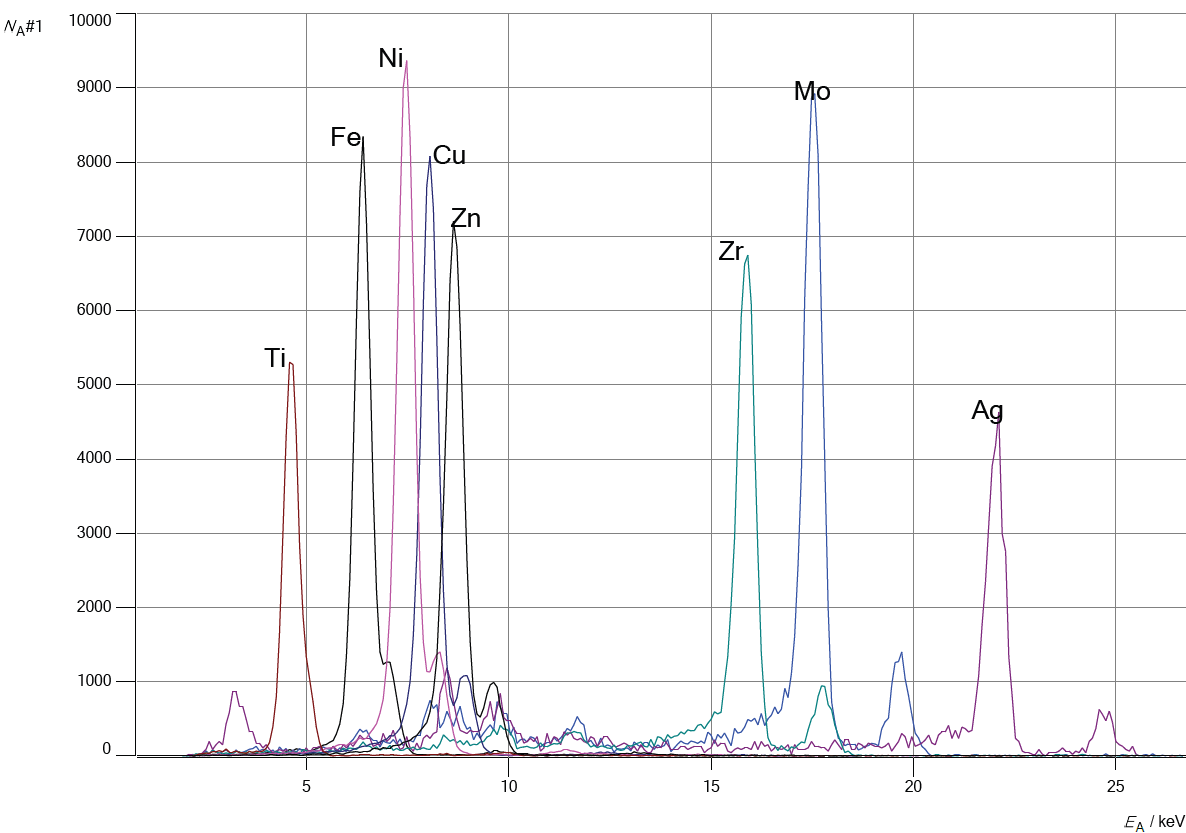
\includegraphics{graphics/aufnahmen/alle_metalle.png}}
    \caption{Gemessene Spektren aller Metallplättchen}
    \label{fig:Metallplatten}
\end{figure}

\begin{figure}[!p]
    \centering
    \resizebox{\textwidth}{!}{
    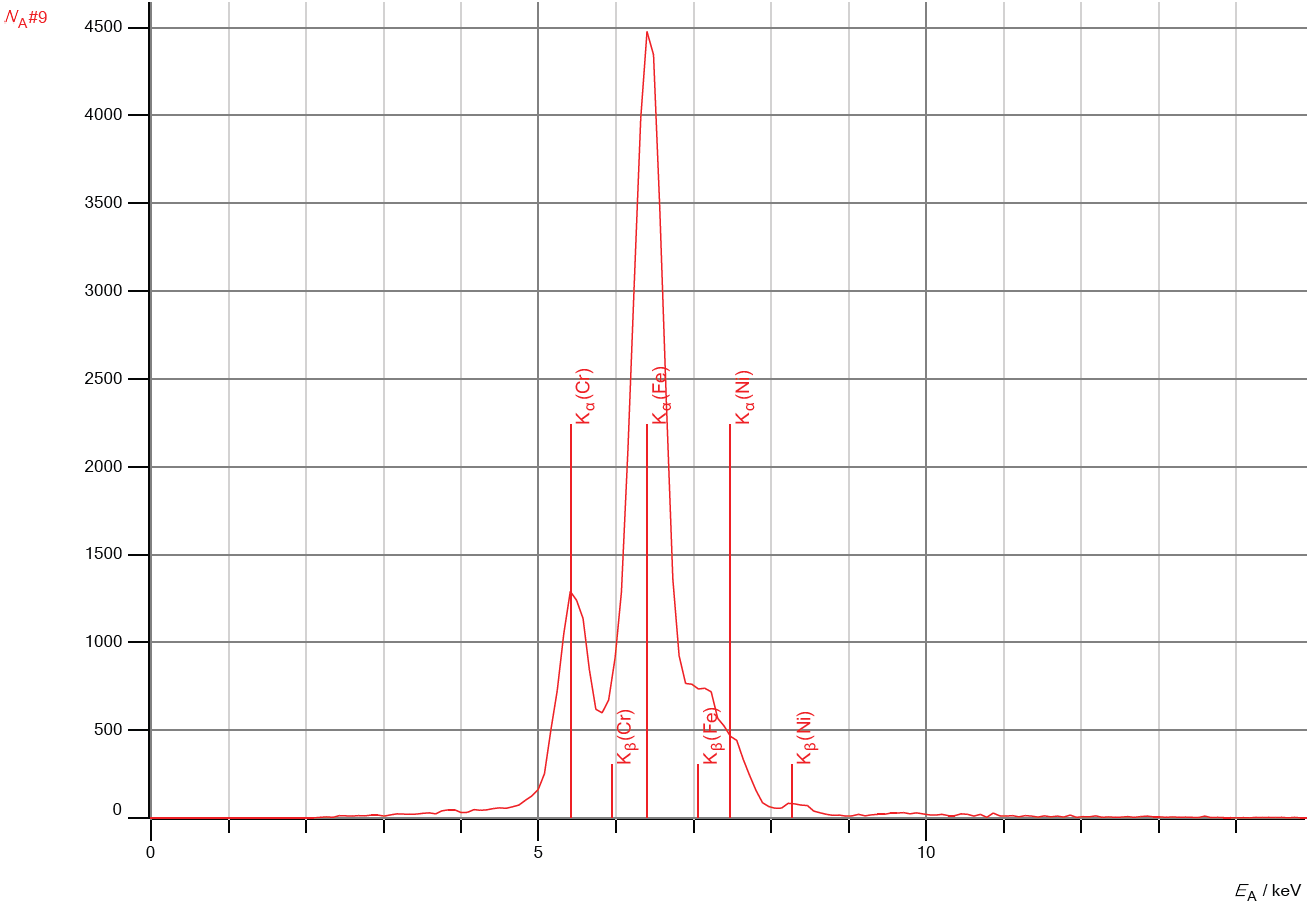
\includegraphics{graphics/aufnahmen/leg1.png}}
    \caption{Gemessenes Spektrum der Legierung (Probe 1)}
    \label{fig:Legierung}
\end{figure}

\begin{figure}[!p]
    \centering
    \resizebox{\textwidth}{!}{
    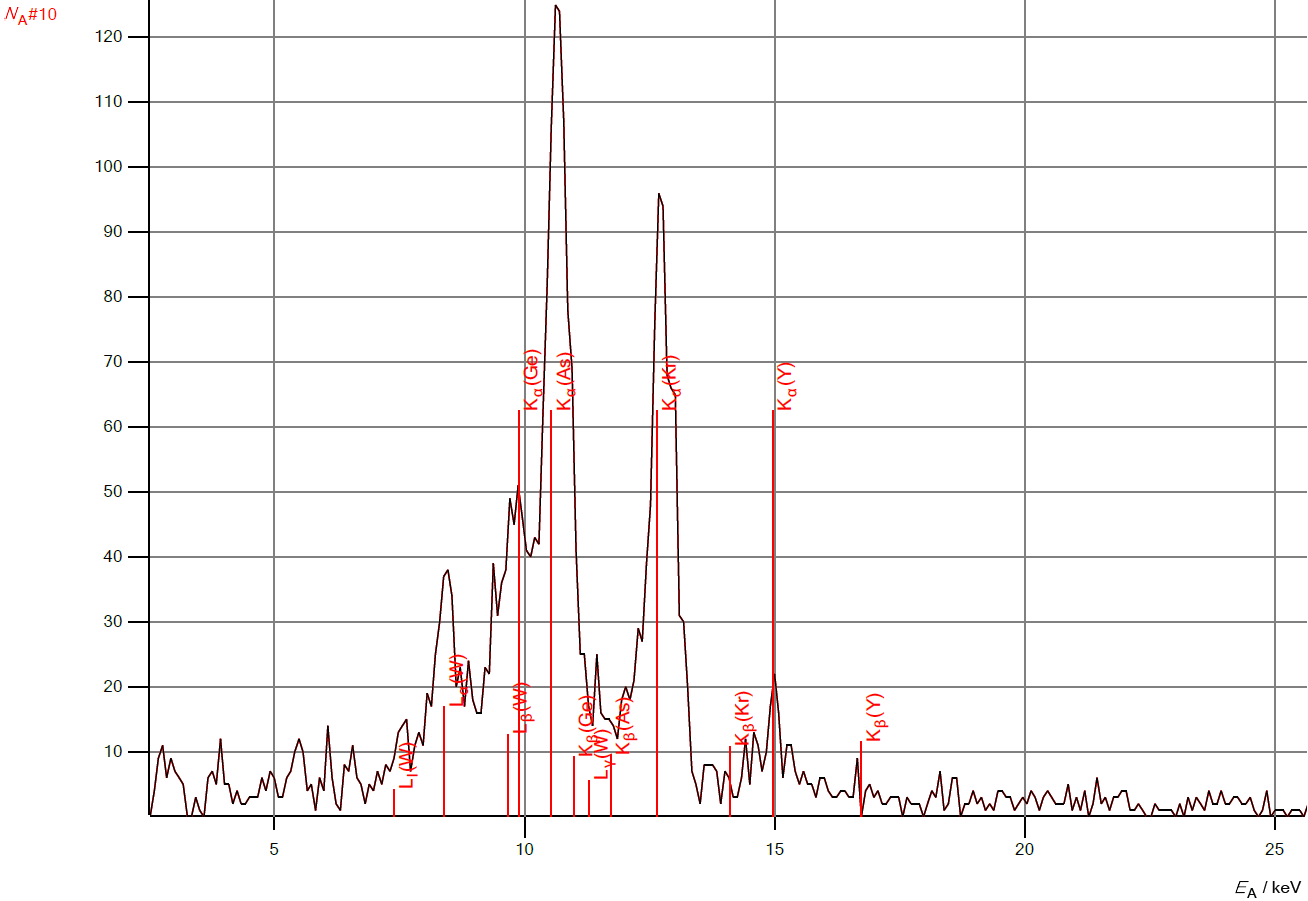
\includegraphics{graphics/aufnahmen/magnet.png}}
    \caption{Gemessenes Spektrum des Magnets}
    \label{fig:Magnet}
\end{figure}

\begin{figure}[!p]
    \centering
    \resizebox{\textwidth}{!}{
    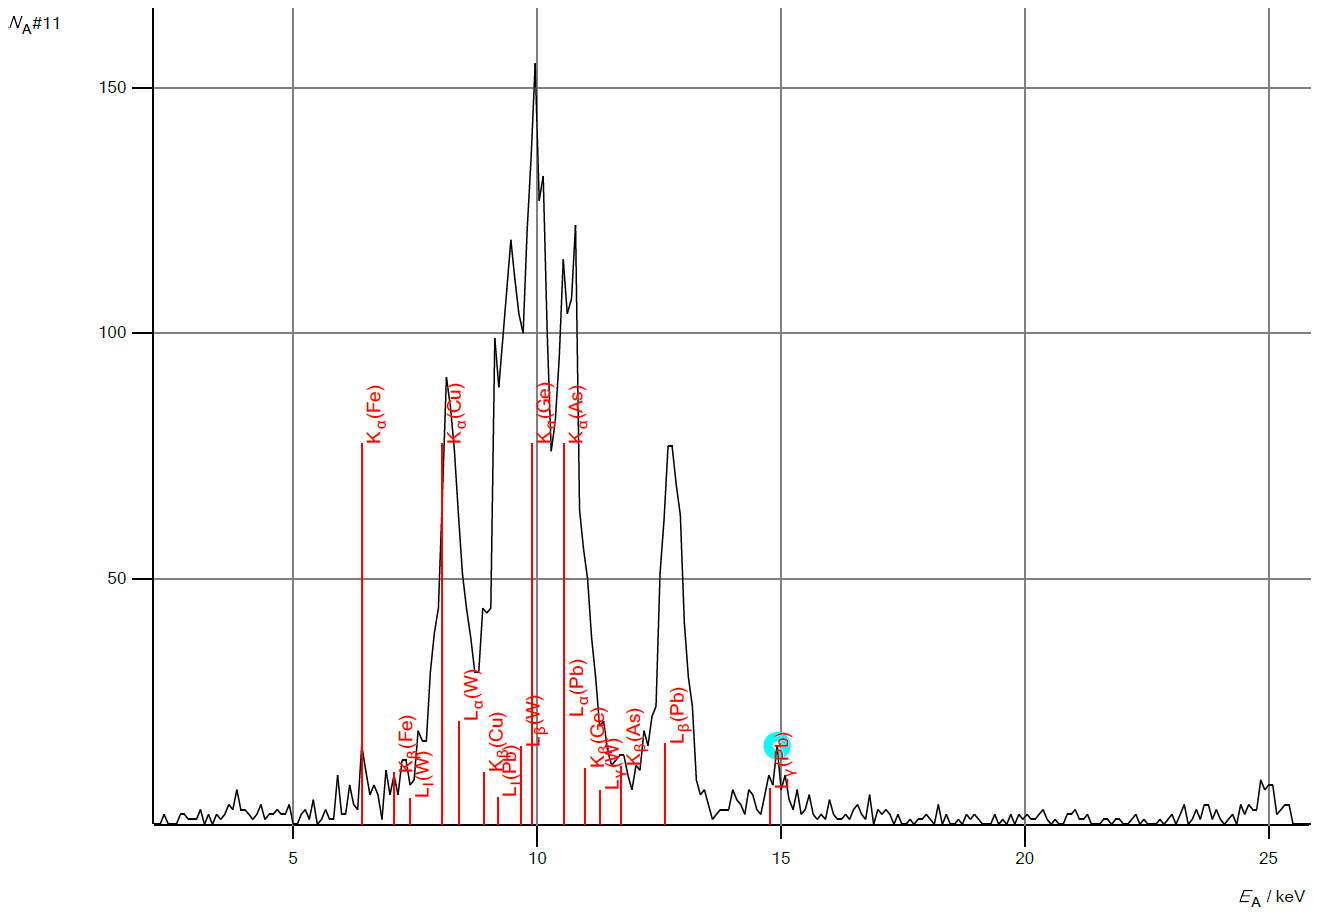
\includegraphics{graphics/aufnahmen/pulver.png}}
    \caption{Gemessenes Spektrum der Pulvermischung}
    \label{fig:Pulvermischung}
\end{figure}

\clearpage
\newpage

\addtocounter{table}{2}

%-------------------------AUSWERTUNG-------------------------
\section{Auswertung}

In dieser Evaluation werden alle Fehler, sofern keine spezifische Angabe gemacht wird, mithilfe der Gauss'schen Fehlerfortpflanzung berechnet. Dies bedeutet, dass ein Wert $F$, der mit der Formel $f(a_1, ..., a_n)$ berechnet wird, den Fehler $\Delta F$ annimmt:

\begin{equation}
    \Delta F = \sqrt{\sum_n \left( \frac{\partial f}{\partial a_n} \cdot \Delta a_n \right)^2}.
\end{equation}

Des Weiteren erfolgen Signifikanztests von zwei Werten $a$ und $a'$ über die folgende Formel:

\begin{equation}
    \sigma = \frac{|a-a'|}{\sqrt{(\Delta a)^2 + (\Delta a')^2}}.
\end{equation}

Die Auswertung sowie Berechnung erfolgen über das dem Dokument angehängte Python-Programm.

\newpage

\subsection{Auswertung der gemessenen K-Linien}

Wir beginnen, indem wir die Wurzel der gemessenen K$_\alpha$-Linien aller Metalle aus Tabelle 1 gegen die zu den Metallen gehörenden Kernladungszahlen $Z$ in ein Diagramm auftragen. An den so linear entstehenden Verlauf passen wir mithilfe der 'curve\_fit' Funktion des Scipy-Packages in Python die folgende Funktion basierend auf dem Moseley'schen Gesetz an:

\begin{equation}
    \sqrt{E_\alpha} = \sqrt{E_R} (Z - \sigma_{12}) \sqrt{\frac{1}{n_1^2} - \frac{1}{n_2^2}}.
\end{equation}

\begin{figure}[!b]
    \centering
    \resizebox{0.9\textwidth}{!}{
    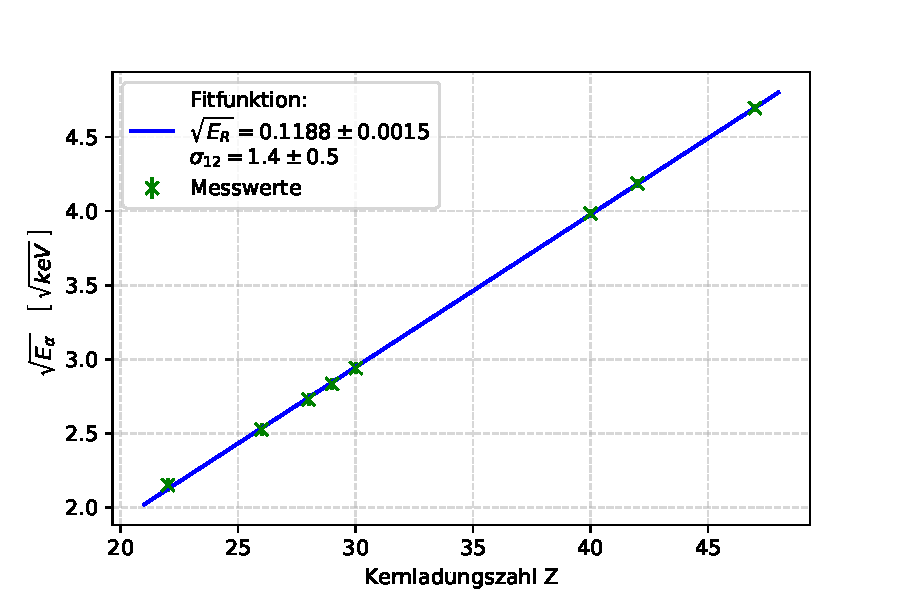
\includegraphics{graphics/Ka.pdf}}
    \caption{Messdaten der K$_\alpha$-Linien}
    \label{fig:Ka_Plot}
\end{figure}

Für $n_1$ und $n_2$ wählen wir die zum K$_\alpha$-Übergang gehörenden Quantenzahlen $n_1 = 1$ und $n_2 = 2$. Unser in Abbildung \ref{fig:Ka_Plot} dargestellte Fit ergibt dabei die Werte

\begin{equation}
    \begin{split}
        \sqrt{E_R} &= (0,1188 \pm 0,0015) \sqrt{\text{keV}} \\ \\
        \Rightarrow \bm{E_R} &\bm{= (14,1 \pm 0,4)} \textbf{eV} \\ \\
        \bm{\sigma_{12}} &\bm{= 1,4 \pm 0,5}
    \end{split}
\end{equation}

\newpage

Wir vergleichen den Wert für die Rydbergenergie $E_R$ mit dem Literaturwert $E_{R,lit} = 13,605693$eV und die Abschirmungskonstante $\sigma_{12}$ mit dem häufig verwendeten Näherungswert 1. Wir erhalten die folgenden Abweichungen:

\begin{equation}
    \begin{split}
        \sigma_{E_R} &= 1,41 \\
        \sigma_{\sigma_{12}} &= 0,77
    \end{split}
\end{equation}

Beide Abweichungen liegen innerhalb des $3\sigma$-Bereichs und sind somit nicht signifikant. Es ist jedoch auffällig, dass die Abschirmungskonstante mit 1,4 größer ist als der häufig als Näherung verwendete Wert 1, was ein erstes Anzeichen darauf ist, dass es eine sehr grobe Näherung ist.  

Wir wiederholen die gleiche Auswertung für die gemessenen Energien der K$_\beta$-Linien. Zu beachten ist, dass beim K$_\beta$-Übergang nun $n_2 = 3$ gilt. Der Fit, zu sehen in Abbildung \ref{fig:Kb_Plot}, ergibt diesmal die folgenden Werte:

\begin{equation}
    \begin{split}
        \sqrt{E_R} &= (0,1176 \pm 0,0013) \sqrt{\text{keV}} \\ \\
        \Rightarrow \bm{E_R} &\bm{= (13,8 \pm 0,3)} \textbf{eV} \\ \\
        \bm{\sigma_{13}} &\bm{= 2,1 \pm 0,4}
    \end{split}
\end{equation}

\begin{figure}[!h]
    \centering
    \resizebox{0.8\textwidth}{!}{
    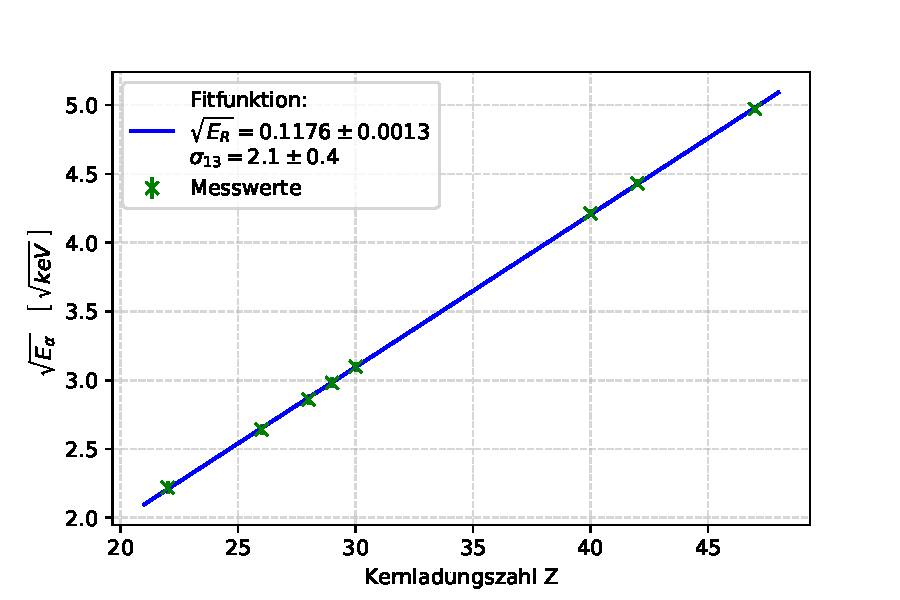
\includegraphics{graphics/Kb.pdf}}
    \caption{Messdaten der K$_\beta$-Linien}
    \label{fig:Kb_Plot}
\end{figure}

\newpage
Analog vergleichen wir mit den Literatur- beziehungsweise Näherungswerten und erhalten:

\begin{equation}
    \begin{split}
        \sigma_{E_R} &= 0,72 \\
        \sigma_{\sigma_{13}} &= 2,66
    \end{split}
\end{equation}

Erneut sind zwar beide Abweichungen theoretisch innerhalb der $3\sigma$-Umgebung, jedoch sind hier insbesondere bei der Abschirmungskonstante deutliche Abweichungen vom Wert 1 zu erkennen. Mit einem Wert von 2,1 bestätigt sich die bereits bei den K$_\alpha$-Linien gemachte Beobachtung, das die Näherung der Abschirmungskonstante mit 1 eine sehr grobe ist. Abseits davon ergibt sich für die Rydbergenergie ein besseres Ergebnis als bei den K$_\alpha$-Linien, was sich aber nicht direkt mit gröberen Fehlern oder Ursachen in Verbindung setzen lässt. 

\subsection{Kommentar zur Analyse der Zusammensetzung der Proben}

Die in den Abbildungen \ref{fig:Legierung} bis \ref{fig:Pulvermischung} dargestellten Spektren wurden in der Durchführung im verwendeten Programm CASSY Lab 2 mit den Linien der zugeordneten Elemente ergänzt. Die gefunden Zusammensetzungen waren:

\begin{itemize}
  \item Legierung: Eisen, Chrom und Nickel.
  \item Magnet: Germanium, Arsen, Yttrium, Wolfram und Krypton.
  \item Pulvermischung: Eisen, Kupfer, Germanium, Arsen, Wolfram und Blei.
\end{itemize}

Diese Zusammensetzungen erscheinen bei der Legierung und der Pulvermischung recht sinnvoll. Lediglich beim Magnet scheint sich eine nicht ganz sinnvolle Zuordnung untergemischt zu haben. Die Auswahl von Krypton motiviert durch die starke Linie bei ca. 12,5keV erscheint zwar zunächst passend, wird jedoch schnell fragwürdig wenn man bedenkt dass Krypton ein Edelgas ist und somit höchstwahrscheinlich nicht in einem handelsüblichen Magnet vorkommt. Jedoch wirken die Alternativen wie beispielsweise die K$_\beta$-Line von Selen mit einer Energie von 12,5keV oder die K$_\alpha$-Linen der benachbarten Elemente von Krypton, Brom und Rubidium, auch nicht gerade sinnvoller im Kontext der Zusammensetzung eines Magnets, weshalb es schwer ist hier eine sichere Alternative für die stark ausgeprägte Linie zu nennen.




\newpage
%---------------PRÄSENTATION DER ENDERGEBNISSE---------------
\section{Zusammenfassung der Endergebnisse}

In diesem Versuch untersuchten wir die Röntgenspektren verschiedener Metalle und Proben. Aus den bestimmten Energien der K$_\alpha$ und K$_\beta$-Linen verschiedenster Materialien bestimmten wir die Rydbergenergie sowie die Abschirmungskonstante. Bei den K$_\alpha$-Linen erhielten wir

\begin{equation}
    \begin{split}
        \bm{E_R} &\bm{= (14,1 \pm 0,4)} \textbf{eV}, \\ \\
        \bm{\sigma_{12}} &\bm{= 1,4 \pm 0,5}.
    \end{split}
\end{equation}

Diese Ergebnisse wiesen im Vergleich zu Literatur- beziehungsweise Näherungswerten insignifikante Abweichungen auf, wobei der erhöhte Wert der Abschirmungskonstante bereits auf einen groben Näherungswert vorahnen ließ.

Bei den K$_\beta$-Linen kamen wir auf die folgenden Werte:

\begin{equation}
    \begin{split}
        \bm{E_R} &\bm{= (13,8 \pm 0,3)} \textbf{eV}, \\ \\
        \bm{\sigma_{13}} &\bm{= 2,1 \pm 0,4}.
    \end{split}
\end{equation}

Hier war nun die deutliche Abweichung der Abschirmungskonstante vom Näherungswert 1 sichtbar, was sich auch in einer erhöhten Sigmaabweichung sichtbar machte, die nur aufgrund des relativ hohen Fehlers des Fitparameters noch innerhalb der $3\sigma$-Umgebung blieb. Somit war nun eindeutig, dass die Näherung im allgemeinen nicht korrekt ist und stark von der Realität abweicht. Der Wert der Rydbergenergie war aber dafür umso besser und lag sogar näher am Literaturwert als der vorher über die K$_\alpha$-Energien berechnete Wert. 

Zuletzt betrachteten wir die Analyse der Zusammensetzung der Proben und stellten fest, dass alle Zuordnungen bis auf eine sinnvoll erscheinen und auch im Kontext der jeweiligen Probe realistisch erscheinen. Für die eine als fehlerhaft bewertete Zuordnung wurden verschiedene Alternativen untersucht, woraufhin jedoch keine endgültige Alternative gefunden werden konnte.   


\newpage
%---------------ZUSAMMENFASSUNG UND DISKUSSION---------------
\section{Diskussion}

Die Ergebnisse der Auswertung zeigen größtenteils ein einstimmiges Bild: Die Rydbergenergie konnte beide Male ohne große Probleme bestimmt werden und die Näherung der Abschirmungskonstante mit 1 weicht schnell sehr stark von der Realität ab. Wir möchten nun kurz die Versuchsdurchführung kommentieren und auf gegenenfalls entstande Fehlerquellen sowie Verbesserungsmöglichkeiten eingehen.

Das Aufnehmen der Spektren verlief eigentlich problemlos und die digitale Einstellung des Geräts sowie die darauffolgende digitale Aufzeichnung minimieren menschliche Fehler. Ebenso wurden die Spektren danach digital im Programm direkt geeicht und in diesem ausgelesen, sodass sich auch hier die Messfehler minimieren und es keine größeren Fehlerquellen gibt. Auch die analyse der Spektren der Proben sowie deren Zusammensetzung erfolgte komplett digital in CASSY Lab 2. Somit lassen sich als potentielle Fehlerquellen eigentlich nur statistische Fehler an den Messgeräten oder der Röntgenröhre nennen. 

Alternativ lassen somit größere Abweichungen nur auf eventuelle Fehler in den verwendeten Formeln schließen, insofern man gröbere Schwankungen der Messgeräte ausschließt. Hier könnten Aspekte wie die Annäherung über das Bohr'sche Atommodell oder die Zusammenfassung der beiden einzelnen Abschirmungskonstanten zu einem $\sigma_{12}$ für Abweichungen von Literaturwerten sorgen.

Bei der Zuordnung der Zusammensetzung hätte eine ausführlichere Auseinandersetzung mit den theoretisch zu erwartenden Elementen für eine klarere Identifizierung der Linien und weniger unwahrscheinlich scheinende Ergebnisse gesorgt.   

Abschließend lässt sich aber allgemein sagen, dass größtenteils positive und aussagekräftige Ergebnisse erzielt wurden und der Versuch somit im Kontext des Anfängerpraktikums eine lehrreiche und interessante Erweiterung zum vorangegangenen Versuch der Röntspektroskopie darstellt. 


\newpage
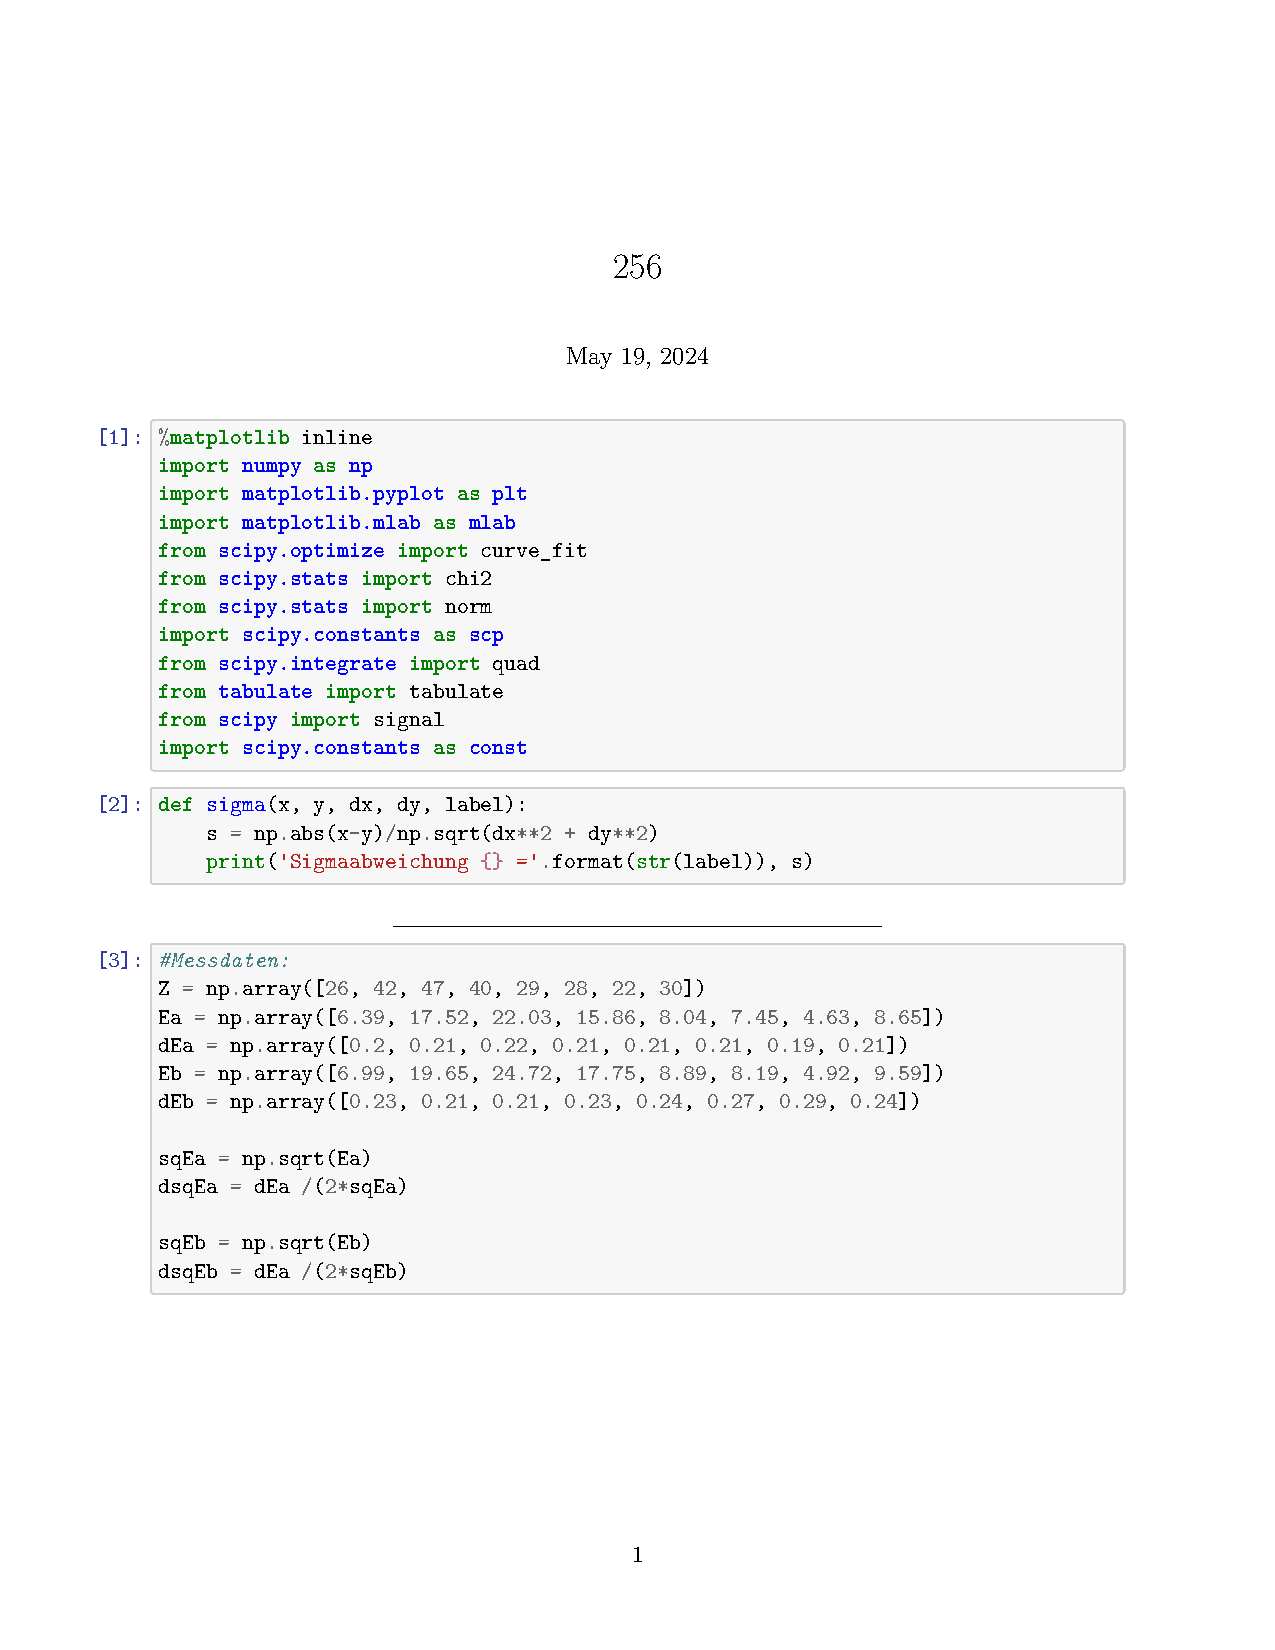
\includepdf[pages=-]{256.pdf}

\end{document}

